\documentclass[11pt]{article}
\usepackage[margin=1in]{geometry}
\usepackage{stfloats} 
\usepackage{graphicx}
\usepackage[superscript,biblabel]{cite}
\usepackage{url}
\usepackage[font={small},margin={.2in},labelfont+={it}]{caption}
\usepackage{subcaption}
\twocolumn
\flushbottom
\begin{document}
\author{Daniel Speyer\\dls2192 \and Samuel Lee\\hsl2113 \and Peiran Hu\\ph2439}
\title{SpatialTable: A Distributed Database for Multidimensional Queries}

\pretolerance=8000


\maketitle

\begin{abstract}
Both spatial databases and distributed databases have proved useful for a variety of problems.  Furthermore, it is possible, albeit inelegant, to store spatial data in a nonspatial distributed database by means of Geohashing and this has proved useful as well.  We propose a natively spatial distributed database, and evaluate its performance.  While it is not as performant as the existing best-of-class solution in the most common case, it is superior in several other cases.  Finally, we make the claim that these cases are important, and therefore that natively spatial distributed databases are worth pursuing.
\end{abstract}

\section{Related Work}

\subsection{Distributed Databases}

The current standard for distributed databases begins by having a single primary key (usually a string) and arbitrary data. The table is sorted by the key, and chopped into ``tablets'' of consecutive rows. Which tablet is on which server is stored in a metadata table, which is part of the database and fits this structure nicely. This makes it easy to search by key, or for a range of keys, but to search for anything else requires either a separate index or reading through the entire table.

\subsection{Spatial Databases}

There exist many single-node spatial databases, mostly based on rtrees\cite{rtrees}, quadtrees\cite{quadtrees}, or similar structures\cite{samet}. They are widely used in geographic applications, as a single node can hold a fairly large amount of data. Still, like all single-node systems, they have a cap on their scalability, and they are not robust against hardware failure.

\subsection{GeoHashing}

\begin{figure}[b!]
\centering
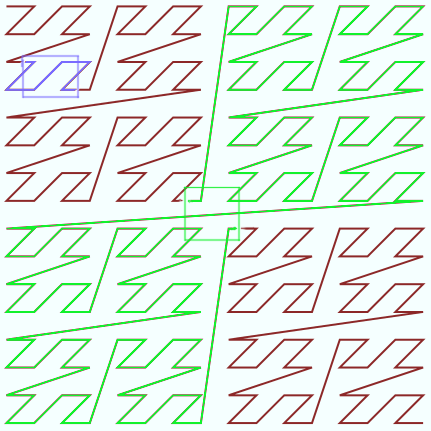
\includegraphics[width=3in]{geohash}
\caption{A 4th degree z curve, showing two queries and their respective linearizations.  The blue query has only 50\% overhead, whereas the green has over 30x}
\label{fig:z}
\end{figure}

Geohashing allows 2-dimensional data to be mapped to a one dimensional key with some locality preserved.  Conceptually, a finite fractal ``z'' shape is drawn over the space, and every point in the space is mapped to the closest point on the fractal.  Note that this requires both the range and precision of the data to be known at index-construction time.  The distance along the fractal provides a scalar descriptor of the location.  This can be used as a primary key in a classic distributed database.\cite{gh}

A query in 2-space can then be translated into an approximate query in z-space.  Given a box, it is computationally straightforward to find the first and last points along the z-curve that are inside the box.  Then all points inside the box must also have z values between those two points.  Not all values between those points must be inside the box, but for most queries, most of them will be.  Specifically, the expected overhead grows logarithmically in the size of the total database\cite{ghs}.  This is illustrated in figure \ref{fig:z}. A database can then scan between the points and filter for being inside the box, with good expected (but poor worst-case) efficiency.

\subsection{Hyperspace Hashing}

Hyperspace hashing is another multidimensional technology. First, each key attribute is `hashed' (the reason for the scare quotes will become apparent). These hashes are then treated as axes of a geometric space, which is statically broken into hyperrectangles (called ``regions'') which are statically assigned to servers.\cite{hh}

According to the original hyperdex paper, the system scales poorly with a high number of regions. Since regions grow exponentially with dimension, hyperdex recommends that dimen\-sionality be kept low, and high-dimension tables be divided into `subspaces' using replication. The system does offer transactions in this replication, though one must worry about the robustness of such a complex system. Also, it requires all the data to be stored once per subspace. Furthermore, queries that specify multiple subspaces only get the benefits of indexing for one, and must scan and filter for the others.

While hyperdex does support range queries, it requires that ``objects' relative orders for the attribute must be preserved when mapped onto the hyperspace axis.'' Since these attributes are not being hashed, but the attribute space is still divided statically, the system is at high risk of hot spots unless the data's distribution is well known in advance.

\section{Design}

Rather than layering on top of a 1-dimensional database, our design uses arbitrary-dimensional tablets as first-class members, giving full flexibility of dimension, range, resolution and distribution with no scan-and-filter needed for standard queries.

\subsection{General Design}

Our design is largely inspired by Google's Bigtable\cite{bigtable}. Like Bigtable, we divide our table into tablets, keep our metadata in a table like the original one, and cap the recursion at two levels. Also, like bigtable, we use a general distributed filesystem (hdfs) as our backing store.

Our system is intended as a proof-of-concept, not a production-ready system. As such, we do not support true statelessness as bigtable does, but store data in RAM and write to hdfs eventually. As such, we are not robust against node failures, but the technologies of write-ahead logging and compactions are already well-established, and we would discover nothing new by re-implementing them.

We did consider implementing our system as an add-on to hbase (an existing open source distributed database) but the codebase there was too large and insufficiently documented, so this was not practical.

In a later section, we discuss both what would be necessary to render our system production-ready, and what would be necessary to merge it with an existing database.

Since we want to use our same technology for metadata, and the natural shape for tablets is hyperrectangles (henceforth known as ``boxes'' for brevity), the keys to our rows are boxes as well. The data associated with the row is an arbitrary binary blob. For our tests, we used strings, but a user is welcome to put protobufs there (as we do for metadata). Supporting bigtable-like columns would again be a practical feature of no research significance.

\subsubsection{Tablets}

Each tablet has borders (a box) and optionally a list of perpendicular hyperplanes through that box which all entries inside the tablet must cross.  For brevity, we refer to these hyperplanes as ``lines'', which they are in the 2-dimensional case.   Since all the lines must be perpendicular, there can be at most as many lines as dimensions. In this all-lines case, all entries inside the tablet must contain a single point. The borders of the box may include infinity or negative infinity. An entry from (1,1) to (2,3) would qualify as inside of a tablet from (0,0) to (5,3) but would not qualify as crossing a line at dim$_0$=2.

This definition, combined with the splitting algorithm, allows us to maintain a vital invariant: for any possible entry, there is always exactly one tablet that should contain it.

\subsubsection{Splitting}

When a tablet becomes too large, we split it along one dimension, producing three tablets: `less', `crossing' and `more'. The `less' and `more' tablets have smaller borders and the same (if any) lines which must be crossed. The `crossing' tablet has the same borders, but a new line where the split occurred. Entries are then assigned to the new tablets based on how they relate to the split line in that dimension.

\begin{figure}[h]
\centering
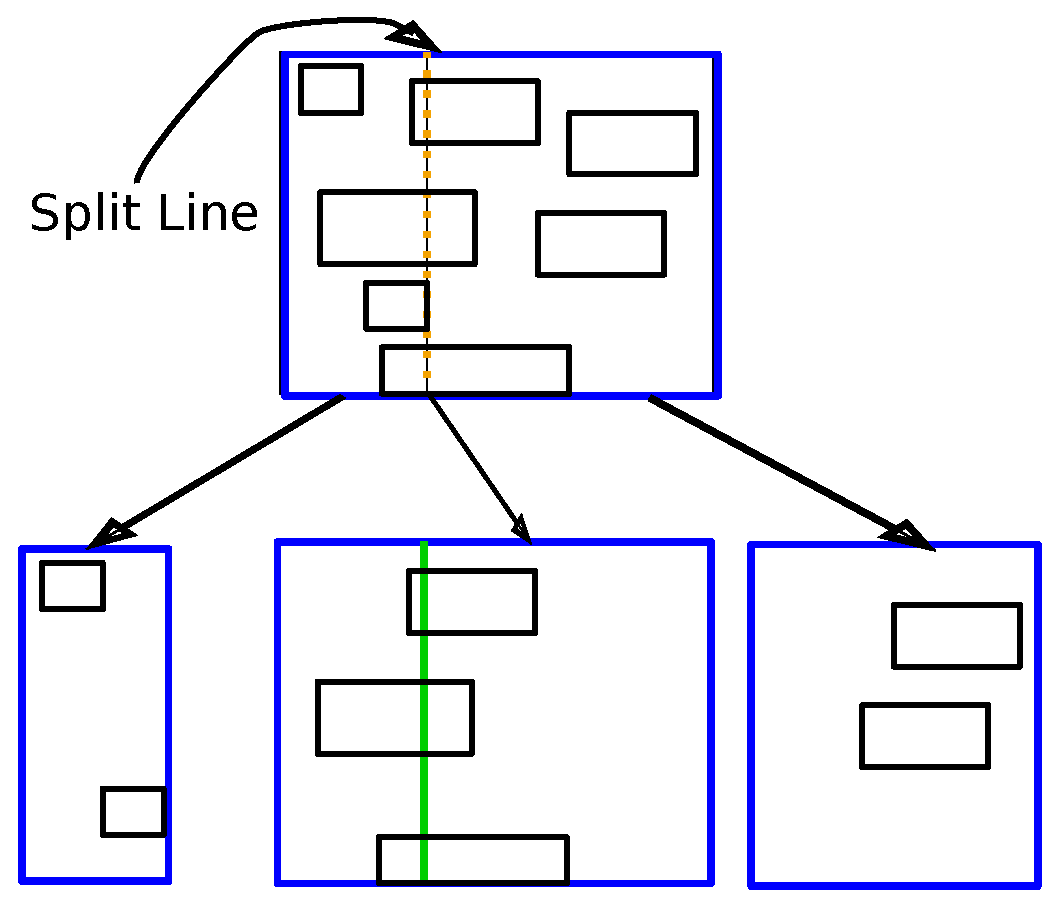
\includegraphics[width=2.5in]{tabsplit}
\caption{Splitting a 2d tablet}
\label{fig:split}
\end{figure}

Note that the `less' and `more' tablets have never-before-seen borders, and the `crossing' tablet has the same borders as the tablet which was just destroyed. This pattern ensures that there will never be two tablets in the same table with the same borders, and therefore that we can safely use the borders as the metadata key.

Finding the split line is a matter for heuristics. The only constraint is that we cannot split a tablet in a dimension for which it already has a must-cross line. Also, it is useless to split a tablet in such a way that all the entries land in the same child tablet. This leaves considerable freedom. Our current heuristic is to take the bounding box of the data actually there, then split it in the widest dimension. To find the point along that dimension at which to split, we take the median after dropping the edges. In practice this works fairly well, but it is neither optimal nor robust against pathological data.

\subsubsection{Finding a Single Entry}

To find a single entry, we look in md0 for metadata tablets that contain the box, ignoring must-cross lines, then we look in each of them for the tablet that contains the box and whose must-cross lines the box does satisfy. This may seem counter-intuitive, but consider a box which in the relevant dimension ranges from 11 to 12, inside a tablet from 10 to 20, inside a metadata tablet from 0 to 30 crossing 15. This is a perfectly valid arrangement, even though the entry could not be placed in the metadata tablet.

The number of metadata tablets that must be looked at is one more than the number of splits that location has gone through. Since splits are equivalent to a binary tree, the expected number of tablets to search is logarithmic in the total number of metadata tablets. There is no balancing mechanism, however, and with pathological data it would be possible to have to search 2/3 of the metadata tablets.

\subsubsection{Conducting a Query}

Queries may be of the form `all boxes within this box' or `all boxes intersecting this box'. In either case, we must search all tablets that intersect the query box. 

\subsubsection{Load Balancer}

The job of the load balancer process is to distribute the "load" of the overall database among the different tablet servers. We have defined the load in our case to be the amount of rows contained in each tablet. We follow a simple algorithm to determine which tablets to move and it is as follows. First, we measure the load in each tablet, but instead of querying each table and counting the number of rows, we make use of the fact that each tablet is an rtree and we simply obtain the size attribute for each rtree which corresponds exactly with the number of rows. Next, we determine which servers have the max and min loads and what is the target number of rows we would ideally like to move to balance the load. It is important to note however, that we do not move individual rows from server to server, but instead move whole tablets. This means that even though we have a target number of rows we would ideally like to move, we still need to search for a tablet that best matches the number of rows we would like to move. If we find one, then we move it from the max loaded server to the min loaded server. If no such tablet can be found, then we do nothing, and wait for the next iteration to hopefully find a better candidate. In our experience, this worked decently well, since we are also leveraging the fact that we are splitting the tablets that get too large and thus have mostly evenly sized tablets.

\subsubsection{Locking}

We have a lock on each tablet name, which is held whenever the tablet is in use (including being created or destroyed).  We also have a lock on the map from names to tablets that the tabletserver maintains, which is held whenever creating or destroying tablets.  These are internal locks within the tabletserver that exist to prevent simulataneous accesses from corrupting the data structures.

There is exactly one circumstance in which a lock is held another is waited on: when splitting a tablet, the original tablet remains locked until the metadata updates are complete.  Since the metadata tree is shallow and acyclic, this cannot produce a cyclic wait nor can a significant fraction of threads be blocked at once, unless there are serious delays in an md0 operation.

This provides a tablet-level linearization guarantee to the user.  Since tablets are not a user-visible structure, this amounts to a row-level linearization guarantee.

\subsection{Test Infrastructure}

Currently our infrastructure consists of a four-node cluster of virtual machines with Ubuntu 14.04 LTS on KVM. Each VM is itself a datanode on our distributed file system Hadoop File System (HDFS)\cite{hdfs}. Our code base is written in C++, using various libraries, and our testing software for comparisons to other database systems was written in Java and Python.

\subsection{Dependencies}

\subsubsection{HDFS}

HDFS is a fault tolerant scalable distributed storage component of the Hadoop distributed high performance computing platform, inspired by the Google File System. We chose this file system because it met our reliability, scalability, functionality, and performance goals, and has a very well documented installation and development API in C++. 

\subsubsection{Boost Geometry}

Rather than implement our own spatial data structures in memory, we rely on the Boost Geometry\cite{boost} library's rtree implementation to hold each tablet. Inconveniently, this uses templates for the dimension, requiring the table dimension to be known at compile time. We can work around this for most purposes using function pointers, but It does limit the dimensionalities we can support.

\subsubsection{Boost Serialization}

Since we were already using Boost Geometry to implement our tablets, it was natural to select Boost Serialization as a way to write our data structures to persistent storage, in our case HDFS. The stated goals of Boost serialization of deconstructing an arbitrary set of C++ data structures to a sequence of bytes fit our needs perfectly, however we quickly realized that the stated goal was in fact still a goal, even when dealing with other Boost libraries such as the Boost Geometry. However, we were able to workaround this incomplete implementation and were able to successfully use Boost Serialization to save our data structures to HDFS.

\subsubsection{Protobuf}

We use Google Protobuf\cite{protobuf} for our wire serialization needs. This is the same library used by hbase and many other distributed systems, so we have a degree of compatibility there.

\subsubsection{RPCZ}

LibRPCZ\cite{rpcz} is an open-source rpc client/server library using protobufs. It offers clean interfaces for both synchronous and asynchronous RPCs.

Unfortunately, it uses a naive round-robin thread scheduler which can cause it to hang if too many RPCs take place before the first one completes. Special thanks to Dmitry Odzerikho of that project for helping us to understand and work around this bug.

\begin{figure*}[t]
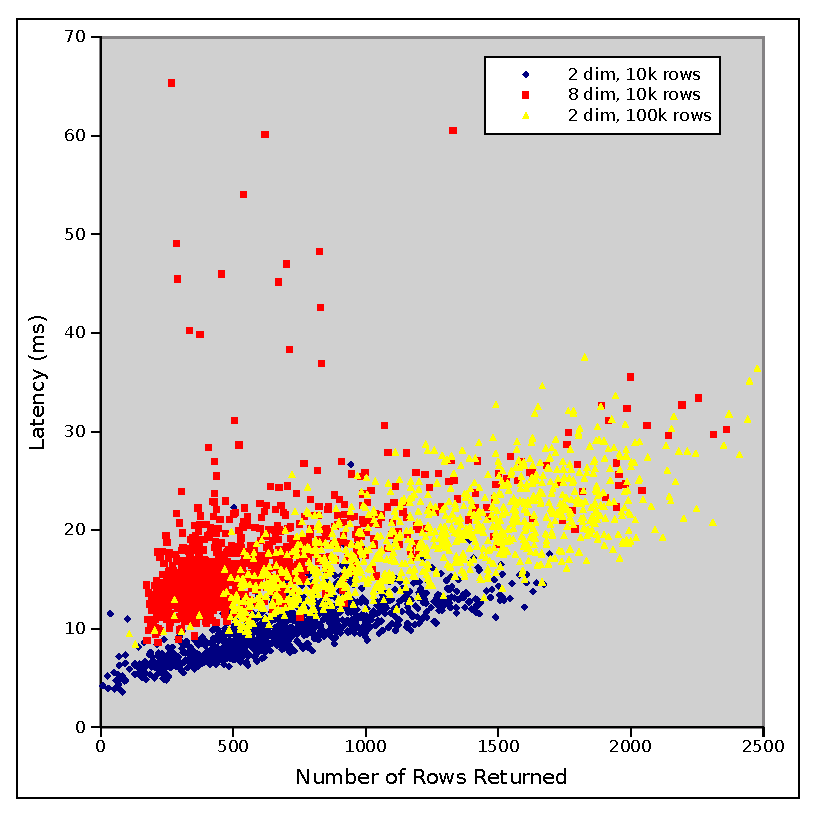
\includegraphics[width=2.1in]{stres}
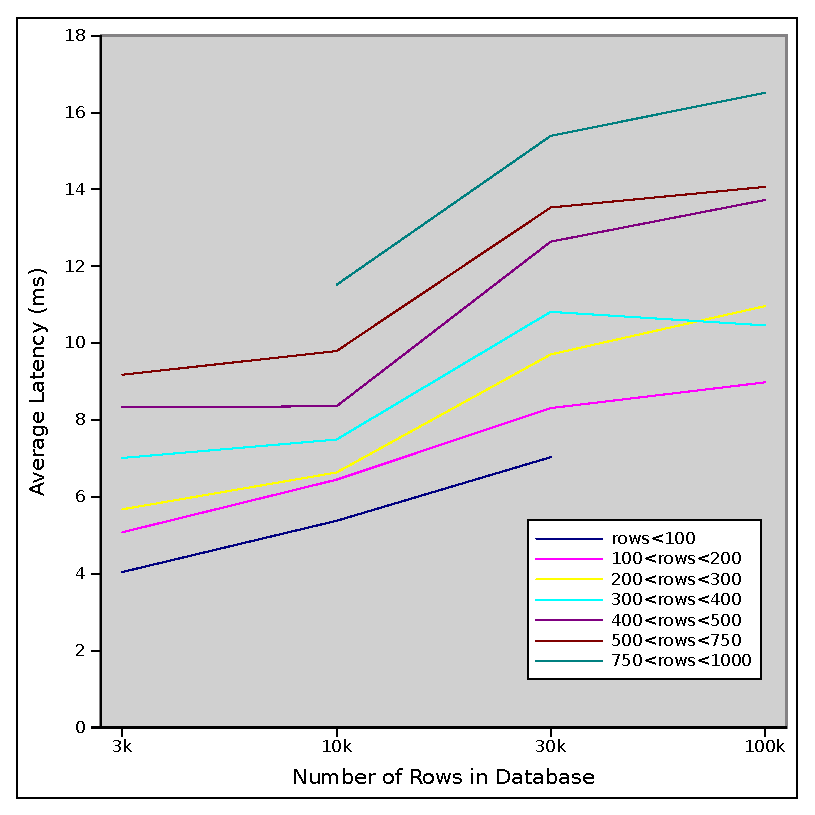
\includegraphics[width=2.1in]{nrowseff}
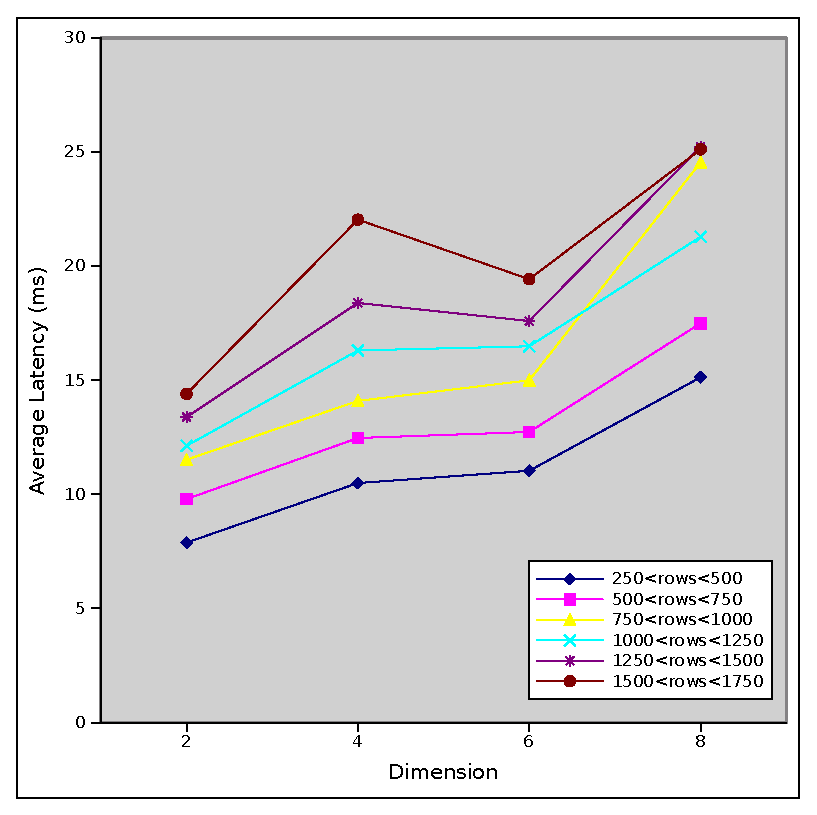
\includegraphics[width=2.1in]{dimeff}
\caption{SpatialTable Performance: (a) Latency vs Rows Returned for individual queries, showing 10k rows of 2 dimensions, 10k rows of 8 dimensions and 100k rows of 2 dimensions; (b) Latency vs Rows in Database, averaged and blocked by rows returned; (c) Latency vs Dimensions, averaged and blocked by rows returned }
\label{fig:res}
\end{figure*}

\section{Results}

\subsection{Description of the Benchmarks}

We do all our benchmarking using queries, because other operations might not be a fair test.  Spatialtable accepts an insertion as soon as the data is in RAM.  Other systems might wait for confirmation from the storage layer.  That would take considerably longer, but not reflect an advantage of our system.

We generate random data using 5 gaussians, spread uniformly across the range $(0,1)$ with $\sigma=0.1$ in all dimensions.  A heatmap of the resulting data is shown in figure \ref{fig:hm}

\begin{figure}[h!]
\centering
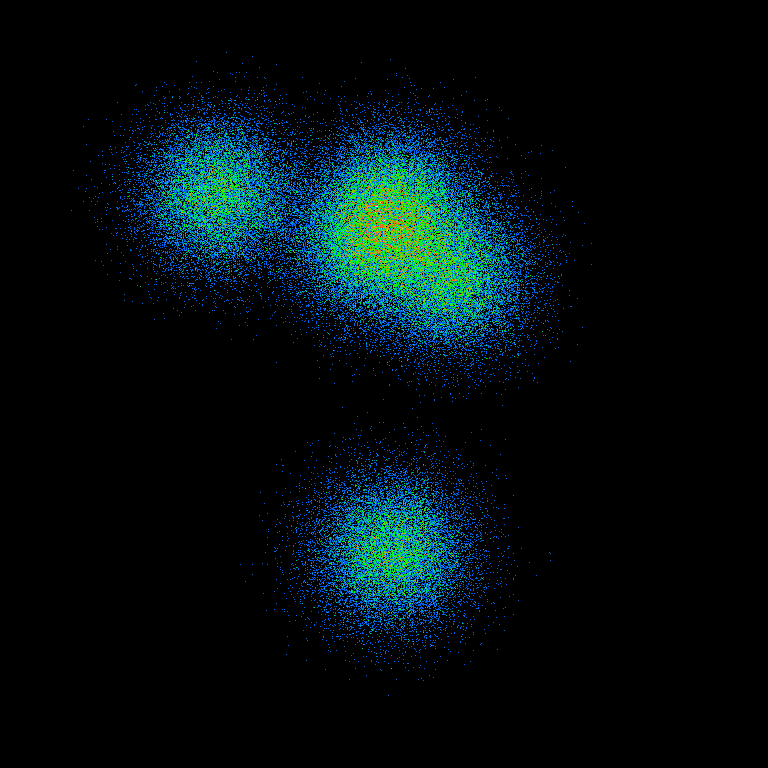
\includegraphics[width=2.5in]{map100k}
\caption{A Heatmap of 100k Random Rows}
\label{fig:hm}
\end{figure}

We then generate random center points for queries using the same distribution.  We select an expected number of results uniformly from the range $(500,2000)$ and create a (hyper)square query to return this.  However, if the query is in a very low-density region of the map, we limit the size of the query so that it does not enter a higher density region, which produces  some queries with significantly fewer results.

\subsection{SpatialTable Performance}

Drawing from a database of 100 thousand 2-dimensional rows using this distribution, SpatialTable has a mean latency of 19ms $(\sigma=4.8)$ with a 95th percentile of 28ms and a maximum (out of our 1000 test queries) of 38ms.

The number of rows returned had a strong effect on latency, every hundred rows costing an extra 0.7ms $(r^2=0.54)$.

The number of dimensions had a weaker effect, each dimension costing about 1.4ms $(r^2\approx 0.8)$.  This is a smaller effect because an extra 200 rows in a response is far more likely than an extra dimension.  Our test at 8 dimensions also showed a significant number of outliers, which our tests at 4 and 6 dimensions did not.   This might be an artifact of the testing.

The size of the total database also has a small effect, with a factor of 10 increase costing about 5ms.  Both the figures for dimension and database-size effect are highly susceptable to change in how they are measured.  The volume of the query box did not effect latency at all.

All of this is illustrated in figure \ref{fig:res}.

\subsection{Comparison to HBase}

\subsection{Comparison to MongoDB with GeoHash}

MongoDB is a popular open-source distributed database with built in geospatial support via geohashing.\cite{mongospatial1}\cite{mongospatial2}  This makes it a natural choice for a comparison.  We compared MongoDB to SpatialTable using 100k rows and the same multigaussian distribution as before.

Mongo is approximately 5ms faster than Spatialtable in the median case, but suffers from high outliers.   At the 95th percentile, performance is roughly even, and at the 99th Spatialtable is almost 20ms faster.  This is shown in more detail in figure \ref{fig:mongo}.

\begin{figure}[h]
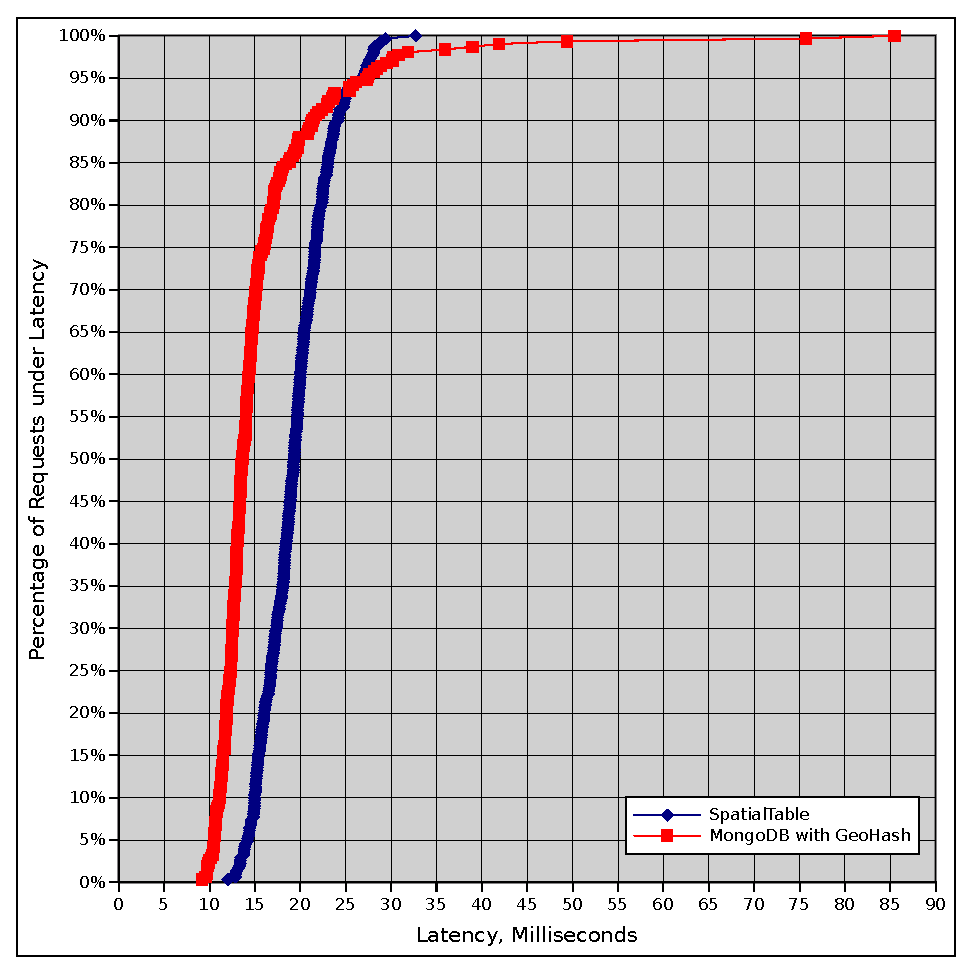
\includegraphics[width=1.55in]{st_mongo_cumu}
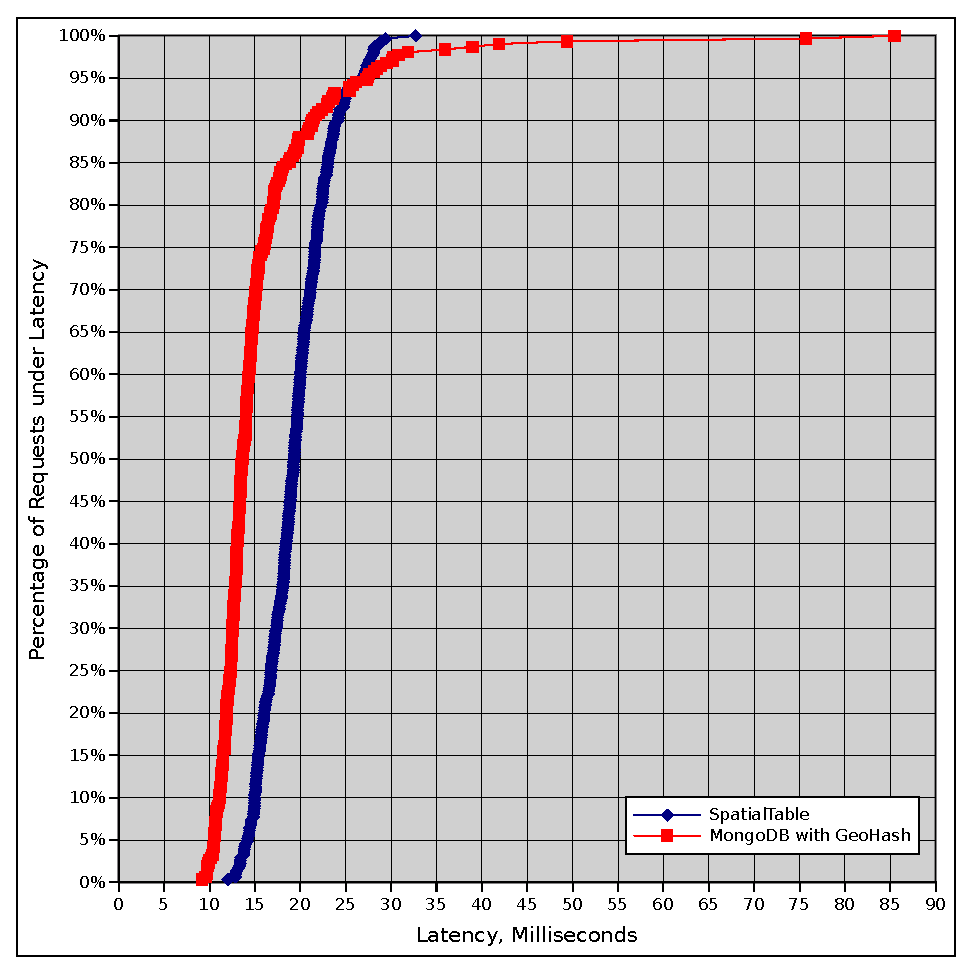
\includegraphics[width=1.55in]{st_mongo_cumu}
\caption{MongoDB vs Spatialtable Drawn from 100k Rows (a) Individual Requests by Rows Returned; (b) Cumulative Histogram for Requests Returning 1000-1500 Rows }
\label{fig:mongo}
\end{figure}

These outliers are exactly what we expect from geohashing in general.  We also expect that a distribution with many points concentrated below the resolution will cause problems.  To trigger this, we reran the test using an exponential distribution.  Each co-ordinate's base 10 log was drawn from a uniform distribution of (-9,9).  We placed the high-density point at the origin to prevent floating point underflow.

With this dataset, we saw a sharp multimodality of MongoDB latencies (see figure \ref{fig:mongoexp}.  The exact nature of this pattern is unclear, but to a first approximation for 38\% of queries the geohashing system worked well, while for the rest it hit resolution issues.  For queries which returned between 1000 and 1500 rows, only 21\% worked well.  The exact numbers are not important, as they are an effect of the exact data chosen, but the lesson is clear: geohashing does not cope well with exponentially distributed data.

\begin{figure}[h]
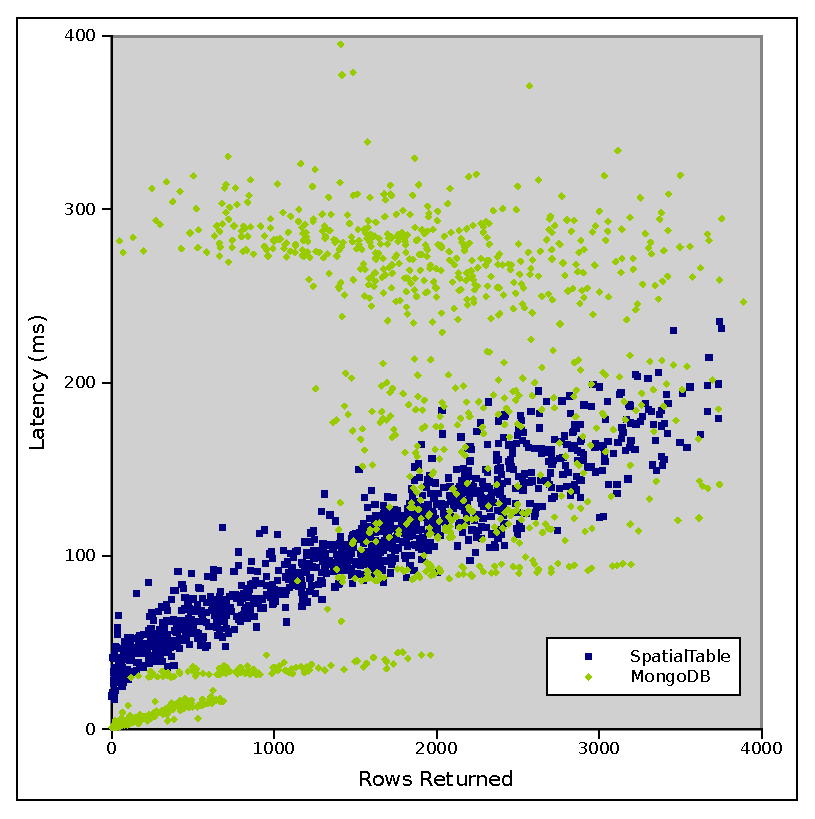
\includegraphics[width=1.55in]{st_mongo_exp}
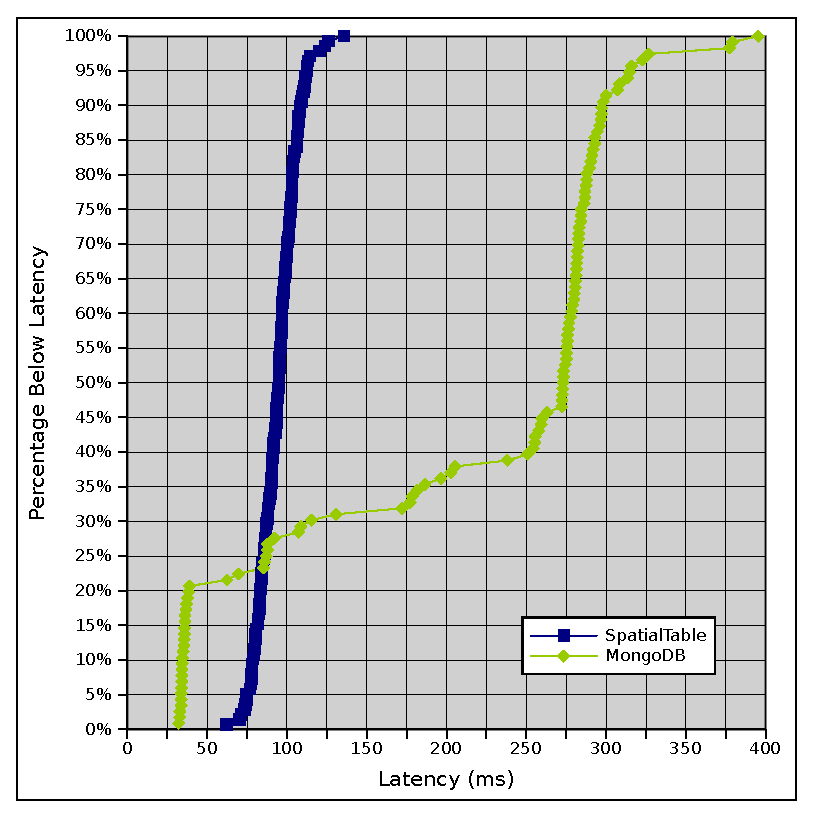
\includegraphics[width=1.55in]{st_mongo_exp_cumu}
\caption{The same graphs as figure \ref{fig:mongo}, but with an exponential distribution of rows}
\label{fig:mongoexp}
\end{figure}

\section{Applications}

For most practical geospatial tasks, geohashing is a good solution.  It is fast, well-suited to gps data on the surface of the Earth, and robustly implemented.  Nevertheless, it suffers from three issues: fixed resolution, strict two dimensionality and high outliers.  We believe there are cases in which these issues are important enough to justify the use of a Spatialtable-like solution instead.

\subsection{High Resolution}

\subsubsection{High Resolution Geospatial}

\subsection{Higher Dimensional}

\subsubsection{Geospatialtemporal}

\subsubsection{DNA ngrams}

Bacterial population studies routinely produce large amounts of data.  A single 16S Ribosomal sequence is only a few kilobytes, but each bacterium in the sample contains at least one copy of that sequence.  The first task in examining such data is often to match each sequence to similar sequences, either in a reference database or in the rest of the sample.  Similarity is defined in terms of alignment, which is very computationally expensive.

One way to make the examinations more computationally tractable is to use ngrams.  Take all possible sequences of a given length (there are $4^n$) and count how many times they appear in the sequence, including overlapping ones.  Then divide the counts by their sum.  While there is no theoretical guarantee, empirically similar ngram signatures predict similar DNA sequences quite well, even for small $n$.\cite{dna}

One option would then be to create a $4^n-1$ (subtract one because the values sum to 1, so the last one provides no information) dimensional table in SpatialTable and store all the sequences in it.  Then for each new sequence, consider only a small box around it to compute precise alignment scores.

\subsection{High Reliability}

There are circumstances under which the 99th percentile performance is more important than the median.  For example, consider a control system for a swarm of mobile robots. A general increase in database latency harms efficiency, but a single timed out request has the potential to cause physical collisions, damaging the robots or their cargo.  

For a less dramatic example, consider a web service with numerous backends.  Each user query results in parallel queries to all the backends.  The user-perceived latency is determined by the slowest backend.  Even if the queries are in sequence, the anomalously slow ones will account for a large fraction of the total time spent.

There are also psychological reasons to focus on bad-case latencies for any user-facing system.  Intermittent very bad experiences cause more user aggravation than consistently mediocre ones.\cite{needed}  Furthermore, if a handful of users have very bad experiences, those users are likely to be the most vocal, shaping the service's reputation.  Perhaps it is for these reasons that Amazon measures all latencies at the 99.9th percentile\cite{amazon}.

\section{Production Readiness}

\subsection{As a Stand Alone}

\subsubsection{Write ahead Logging}

\subsubsection{Handling Metadata Timeouts}

\subsubsection{Catching Dropped Tablets}

\subsubsection{Discovery and Partition-Resistance}

\subsubsection{Security}

\subsection{As Part of an Existing Database}

\subsubsection{Per-Table Metadata}

\subsubsection{Protocol}

\section{Roles}

\section{References}

\begin{thebibliography}{99}

\bibitem{rtrees}
  Guttman.
  \emph{R-Trees: A Dynamic Index Structure for Spatial Searching.}
  ACM SigMOD.
  1984

\bibitem{quadtrees}
  Finkel and Bentley.
  \emph{Quad Trees: A Data Structure for Retrieval on Composite Keys.}
  Acta Informatica.
  1974

\bibitem{samet}
  Samet.
  \emph{Applications of Spatial Data Structures.}
  Addison Wesley.
  1990

\bibitem{gh}
  Morton.
  \emph{A computer Oriented Geodetic Data Base; and a New Technique in File Sequencing.}
  IBM Technical Reports. 
  1966

\bibitem{ghs}
 Tropf and Herzog
 \emph{Multidimensional Range Search in Dynamically Balanced Trees.}
 Angewandte Informatik.
 1981

\bibitem{hh}
  Escriva, Wong and Sirer.
  \emph{HyperDex: A Distributed, Searchable Key-Value Store.}
  ACM SigCOMM.
  2012

\bibitem{bigtable}
  Changs et al.
  \emph{Bigtable: a distributed storage system for structured data.}
  OSDI.
  2006

\bibitem{mongospatial1}
  \emph{MongoDB Manual: 2d Index Internals.}
  \url{http://docs.mongodb.org/manual/core/geospatial-indexes/}
  2015


\bibitem{mongospatial2}
  \emph{MongoDB Manual: GeoSpatial Tutorials}
  \url{http://docs.mongodb.org/manual/tutorial/build-a-2d-index/}
  2015

\bibitem{dna}
  Sun et al.
  \emph{ESPRIT: estimating species richness using large collections of 16S rRNA pyrosequences.}
  Nucleic Acids Research.
  2009


\bibitem{amazon}
  DeCandia et al.
  \emph{Dynamo: Amazon’s Highly Available Key-value Store.}
  Symposium on Operating Systems Principles.
  2007

\bibitem{hdfs}
Shvachko, et al.
\emph{The Hadoop Distributed File System}
Proceedings of the 2010 IEE 26th Symposium on Mass Storage Systems and Technologies (MSST)
2010

\bibitem{boost}
Schiling, Boris
\emph{The Boost C++ Libraries}
XML Press
2011

\bibitem{protobuf}
Google.
\emph{https://github.com/google/protobuf}
2015

\bibitem{rpcz}
Samet, Nadav
\emph{https://github.com/thesamet/rpcz}
2015

\end{thebibliography}


\end{document}
